\documentclass[twoside]{article}
\usepackage{aistats2016}


\usepackage{hyperref}
\usepackage{url}
\usepackage[utf8x]{inputenc}
\usepackage[english]{babel}
\usepackage{natbib}
\usepackage{nicefrac}
\usepackage{algorithm}
\usepackage{algorithmic}
\usepackage{amsfonts}
\usepackage{graphics}
\usepackage{graphicx}
\usepackage{tikz}
\usepackage{color,soul,amsmath}
\usepackage{amssymb}
\usetikzlibrary{bayesnet}
\tikzstyle{connect}=[-latex]
\tikzstyle{allconnected}=[line width=0.1cm]

%\usepackage{verbatim}
%\usepackage[active,tightpage]{preview}
%\PreviewEnvironment{tikzpicture}
%\usepackage{savetrees}

\def\bbbr{{\rm I\!R}}
\newcommand{\vp}{\vec{\phi}}
\newcommand{\vmu}{\vec{\mu}}
\newcommand{\vf}{\vec{f}}

\newcommand{\I}{\mathcal{I}}


\newcommand{\E}{\mathbb{E}}
\newcommand{\Var}{\mathbb{Var}}
\newcommand{\Cov}{\mathbb{Cov}} 
\newcommand{\vm}{\vec{m}}
\newcommand{\vx}{\vec{x}}
\newcommand{\vr}{\vec{r}}
\newcommand{\vy}{\vec{y}}
\newcommand{\vz}{\vec{z}}
\newcommand{\vY}{\vec{Y}}
\newcommand{\vX}{\vec{X}}
\newcommand{\bx}{\textbf{x}}
\newcommand{\bX}{\textbf{X}}
\newcommand{\bY}{\textbf{Y}}

\newcommand{\bz}{\textbf{z}}
\newcommand{\bw}{\textbf{w}}
\newcommand{\by}{\textbf{y}}
\newcommand{\bL}{\textbf{L}}
\newcommand{\bI}{\textbf{I}}
\newcommand{\vk}{\vec{k}}
\newcommand{\vL}{\vec{\Lambda}}
\newcommand{\xmin}{x_{\min}}
\newcommand{\pmin}{p_{\min}}
\newcommand{\fmin}{f_{\min}}
\newcommand{\hpmin}{\hat{p}_{\min}}
\newcommand{\hqmin}{\hat{q}_{\min}}
\newcommand{\pfmin}{p_{f_{\min}}}
\renewcommand{\vec}{\boldsymbol}
\newcommand{\fun}[1]{\mathsf{#1}}
\renewcommand{\O}{\mathcal{O}}
\newcommand{\GP}{\mathcal{GP}}
\newcommand{\N}{\mathcal{N}}
\newcommand{\Id}{\vec{I}}
\newcommand{\II}{\mathbb{I}}
\newcommand{\IR}{\mathbb{R}}
\newcommand{\bk}{\textbf{k}}
\newcommand{\bK}{\textbf{K}}
\newcommand{\tr}{\operatorname{tr}}
\newcommand{\argmin}{\operatorname*{arg\: min}}
\newcommand{\argmax}{\operatorname*{arg\: max}}
\newcommand{\chol}{\operatorname{\mathsf{C}}}

\newcommand{\data}{\mathcal{D}}
\newcommand{\reals}{\mathbb{R}}
\newcommand{\sX}{\mathcal{X}}
\newcommand{\xst}{x_{\ast}}
\newcommand{\yst}{y_{\ast}}

\usepackage{xspace}
\newcommand{\acr}[1]{\textsc{#1}\xspace}
\newcommand{\gp}{\acr{gp}}
\newcommand{\dpp}{\acr{dpp}}
\newcommand{\us}{\acr{glasses}}

\newtheorem{theorem}{Theorem}
\newtheorem{lemma}{Lemma}
\newtheorem{corollary}{Corollary}
\newtheorem{proposition}{Proposition}
\newtheorem{definition}{Definition}
\newtheorem{proof}{Proof}
\newtheorem{conjecture}{Conjecture}



\graphicspath{{./},{./figs/}}

% If your paper is accepted, change the options for the package
% aistats2016 as follows:
%
%\usepackage[accepted]{aistats2016}
%
% This option will print headings for the title of your paper and
% headings for the authors names, plus a copyright note at the end of
% the first column of the first page.


\begin{document}

% If your paper is accepted and the title of your paper is very long,
% the style will print as headings an error message. Use the following
% command to supply a shorter title of your paper so that it can be
% used as headings.
%
%\runningtitle{I use this title instead because the last one was very long}

% If your paper is accepted and the number of authors is large, the
% style will print as headings an error message. Use the following
% command to supply a shorter version of the authors names so that
% they can be used as headings (for example, use only the surnames)
%
%\runningauthor{Surname 1, Surname 2, Surname 3, ...., Surname n}

\twocolumn[

\aistatstitle{GLASSES: Relieving The Myopia Of Bayesian Optimisation}

\aistatsauthor{ Anonymous Author 1 \And Anonymous Author 2 \And Anonymous Author 3 }

\aistatsaddress{ Unknown Institution 1 \And Unknown Institution 2 \And Unknown Institution 3 } ]

\begin{abstract}
    We present \us: Global optimisation with Look-Ahead through Stochastic Simulation and Expected-loss Search. 
    The majority of global optimisation approaches in use are myopic, in only considering the impact of the next function value; the non-myopic approaches that do exist are able to consider only a handful of future evaluations. 
    Our novel algorithm, \us, permits the consideration of dozens of evaluations into the future. 
    We show that the far-horizon planning thus enabled leads to substantive performance gains in empirical tests. 
\end{abstract}
\section{Introduction} % (fold)
\label{sec:introduction}

Global optimisation is core to any complex problem where design and choice play a role. 
Within Machine Learning, such problems are found in the tuning of hyperparameters \cite{Snoek*Larochelle*Adams_2012}, sensor selection \cite{Garnett*Osborne*Roberts_2010} or experimental design \cite{martinez-cantin_bayesian_2009}. 
Most global optimisation techniques are myopic, in considering no more than a single step into the future. 
Relieving this myopia requires solving the \emph{multi-step lookahead} problem: the global optimisation of an function by considering the significance of the next function evaluation on function evaluations (steps) further into the future. 
It is clear that a solution to the problem would offer performance gains.
For example, consider the case in which we have a budget of two evaluations with which to optimise a function $f(x)$ over the domain $\sX = [0, 1] \subset \reals$. 
If we are strictly myopic, our first evaluation will likely be at 
$x=\nicefrac{1}{2}$, and our second then at only one of $x=\nicefrac{1}{4}$ and $x=\nicefrac{3}{4}$. 
This myopic strategy will thereby result in ignoring half of the domain $\sX$, regardless of the second choice. 
If we adopt a two-step lookahead approach, we will select function evaluations that will be more evenly distributed across the domain by the time the budget is exhausted. 
We will consequently be better informed about $f$ and its optimum.

There is a limited literature on the multi-step lookahead problem.
\cite{osborne_gaussian_2009} perform multi-step lookahead by optimising future evaluation locations, and sampling over future function values. 
This approach scales poorly with the number of future evaluations considered, and the authors present results for no more than two-step lookahead.
\cite{Marchant*Ramos*Sanner*2014} reframe the multi-step lookahead problem as a partially observed Markov decision process, and adopt a Monte Carlo tree search approach in solving it. 
Again, the scaling of the approach permits the authors to consider no more than six steps into the future. 

There is a clear link between the multi-step lookahead problem and that considered in the literature as \emph{batch} Bayesian optimisation. 
The two problems are distinct but related: the multi-step lookahead problem requires the challenging marginalisation over unknown future evaluation \emph{locations}, in addition to the unknown future evaluation \emph{values} also marginalised by batch approaches. 
Similarly to the state-of-the-art in multi-step lookahead, the batch literature provides only poor scaling with the number of evaluations.
\cite{Ginsbourger2009} present results for no more than six simultaneous function evaluations.
\cite{Azimi2011,Azimi2012} use the surrogate model for $f$ to generate `fake' observations and avoid the marginalization step. 
This produce a large accumulation of errors that does not allow the use of these techniques for the collection of large batches.

We propose an algorithm, \us, that provides scaling superior to existing alternatives.


\section{Background and challenge}
\subsection{Bayesian Optimisation with one step look-ahead} % (fold)
\label{sec:bayesian_optimisation}


Let $f: {\mathcal X} \to \bbbr$ be well behaved function defined on a compact subset ${\mathcal X} \subseteq \bbbr^d$. We are interested in solving the global optimization problem of finding $\bx_{M} = \arg \min_{\bx \in {\mathcal X}} f(\bx)$. We assume that $f$ is a \emph{black-box} from which only perturbed evaluations of the type $y_i = f(\bx_i) + \epsilon_i$, with $\epsilon_i \sim\mathcal{N}(0,\sigma^2)$, are  available. Bayesian Optimization is an heuristic strategy to make a series of evaluations $\bx_1,\dots,\bx_n$ of $f$, tipically very limited in number,  such that the the minimum of $f$ is evaluated as soon as possible. \cite{Lizotte_2008}
\cite{Jones_2001}
\cite{Snoek*Larochelle*Adams_2012}
\cite{Brochu*Cora*DeFreitas_2010}

Assume that $n$ points have been gathered so far, having a dataset $\data_0 = \{(\bx_i,y_i)\}_{i=1}^N = (\bX_0,\bY_0)$. Before collecting any new point, a surrogate probabilistic model for $f$ is calculated. This is topically a Gaussian Process (GP) $p(f) = \mathcal{GP}(\mu; k)$ with mean function $\mu$ and a covariance function $k$, and whose parameters will be denoted by $\theta$.  Let $\I_0$ be the current available information: the conjunction of $\data_0$, the model parameters and the model likelihood type.  Under Gaussian likelihoods, the predictive distribution for $y_*$ at $\bx_*$ is also Gaussian with mean posterior mean and variance
$$\mu(\bx_{*}|\I_0) = \bk_{\theta}(\bx_*)^\top[\bK_{\theta} + \sigma^2 \textbf{I}]^{-1}\by \mbox{ and}$$
$$\sigma^2(\bx_*|\I_0)=k_{\theta}(\bx_*,\bx_*)-\bk_{\theta}(\bx_*)^\top[\bK_{\theta}+\sigma^2 \textbf{I}]^{-1}\bk_{\theta}(\bx_*),$$
where $\bK_{\theta}$ is the matrix such that $(\bK_{\theta})_{ij}=k_{\theta}(\bx_i,\bx_j)$,  $\bk_{\theta}(\bx_{*}) = [k_{\theta}(\bx_1,\bx_{*}),\dots,k_{\theta}(\bx_n,\bx_{*})]^\top$ \cite{Rasmussen:2005:GPM:1162254}.  


Given the GP model, we now need to determine the best location to sample. Imagine that we only have one remaining evaluation ($n=1$) before we need to report our inferred location about the minimum of $f$. Denote by $\eta = \min \bY_0$, the current best found value. We can define the loss of evaluating $f$ this last time at $\bx_*$ assuming it is returning $y_*$ as
$$\lambda(y_*)\triangleq \left\{ \begin{array}{lcl}
y_*;             & \mbox{if}  &  y_* \leq \eta \\
 \eta; & \mbox{if}  & y_* > \eta. \\
\end{array}
\right.$$
Therefore the loss corresponds is the new observed minimum, $\min (\eta,y_*)$. Its expectation is 
$$\ \Lambda_1(\bx_*| \I_0) \triangleq \E[ \min (y_*,\eta)]= \int \lambda(y_*)p(y_* |\bx_*,\I_0)dy_*$$
where the subscript in $\Lambda$ refers to the fact that we are considering one future evaluations.  Giving the properties of the GP, $\Lambda_1(\bx_*| \I_0)$ can be computed in closed form for any $\bx_* \in \mathcal{X}$. In particular, for $\Phi$ the usual Gaussian cumulative distribution function, we have that
\begin{eqnarray}\label{eq:expected_myopic_loss}
\Lambda_1(\bx_*| \I_0) &  \triangleq & \eta \int_{\eta}^{\infty} \mathcal{N}(y_*;\mu,\sigma) dy_* \\ \nonumber
& +  & \int_{-\infty}^{\eta} y_* \mathcal{N}(y_*;\mu,\sigma) dy_*  \\ \nonumber
& = &  \eta +(\mu  - \eta) \Phi (\eta ; \mu, \sigma) - \sigma \mathcal{N} (\eta, \mu, \sigma), \nonumber
\end{eqnarray}

where we have abbreviated $\sigma(y_*|\I_0)$ as $\sigma$ and $\mu(y_{*}|\I_0)$ as $\mu$. Finally, the next evaluation is located   where $\Lambda_1(\bx_*| \I_0) $ gives the minimum value. This point can  be obtained by any gradient descent algorithm since analitical expresions for the gradient and Hessian of $\Lambda_1(\bx_*| \I_0)$  exist \cite{osborne_bayesian_2010}. 



% section bayesian_optimisation (end)

% section introduction (end)

\begin{figure*}
\centering
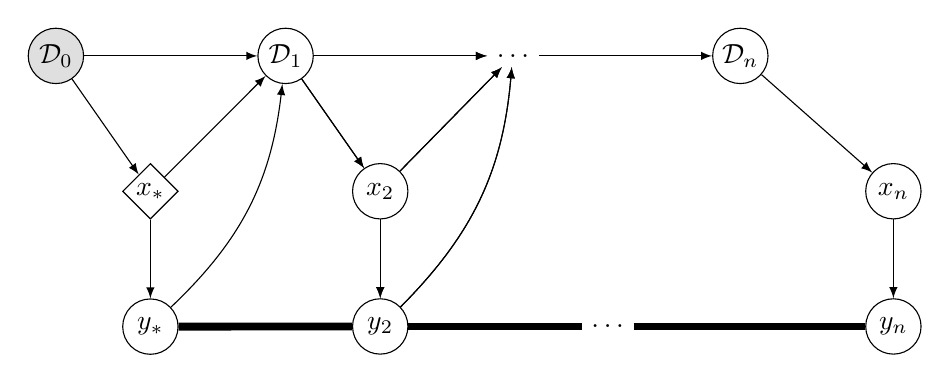
\begin{tikzpicture}

    % first row
    \node[obs] (D0) {$\data_0$};
    \node[latent, right=of D0, xshift=1.2cm] (D1) {$\data_1$};
    \node[draw=none, right=of D1, xshift=1.2cm] (Ddots) {$\ldots$};
    \node[latent, right=of Ddots, xshift=1.2cm] (Dn) {$\data_n$};

    % second row
    \node[det, below=of D0, xshift=1.2cm] (xst) {$\xst$};
    \node[latent, right=of xst, xshift=1.2cm] (x2) {$x_2$};
    \node[latent, right=of x2, xshift=4.8cm] (xn) {$x_n$};

    % third row
    \node[latent, below=of xst] (yst) {$\yst$};
    \node[latent, below=of x2] (y2) {$y_2$};
    \node[draw=none, right=of y2, xshift=1.2cm] (ydots) {$\ldots$};
    \node[latent, below=of xn] (yn) {$y_n$};

    % Connect the nodes
    \path 
        (D0) edge [connect] (D1)
        (D0) edge [connect] (xst)
        (xst) edge [connect] (yst)
        (xst) edge [connect] (D1)
        (yst) edge [connect, bend right=20] (D1)
        (yst) edge [allconnected] (y2)

        (D1) edge [connect] (Ddots)
        (D1) edge [connect] (x2)
        (x2) edge [connect] (y2)
        (x2) edge [connect] (Ddots)
        (y2) edge [connect, bend right=20] (Ddots)
        (y2) edge [allconnected] (ydots)

        (D1) edge [connect] (Ddots)
        (D1) edge [connect] (x2)
        (x2) edge [connect] (y2)
        (x2) edge [connect] (Ddots)
        (y2) edge [connect, bend right=20] (Ddots)
        (ydots) edge [allconnected] (yn)

        (Ddots) edge [connect] (Dn)
        (Dn) edge [connect] (xn)
        (xn) edge [connect] (yn)        
        ;
\end{tikzpicture}
\caption{
    A Bayesian network describing the $n$-step lookahead problem. The shaded node ($\data_0$) is known, and the diamond node ($\xst$) is the current decision variable. All $y$ nodes are correlated with one another under the \gp model.
}
\label{fig:bayes_net}
\end{figure*}


\subsection{Looking many steps ahead and central contribution of this work}
Expression~(\ref{eq:expected_myopic_loss}) can also be used as a miopic approximation to the optimal decision when $n$ evaluations of $f$ remain available. Indeed, most BO methods are myopic and ignore the future decisions that will be made by the algorithm in the future steps. 

Denote by $\{(\bx_j,y_j)\}$ for $j=1,\dots,n$ the remaining $n$ available evaluations and by $\I_j$ the available information after the data set $\data_0$ has been augmented with $(\bx_j,y_j),\dots,(\bx_j,y_j)$ and the parameters $\theta$ of the model updated. We use $\Lambda_n(\bx_*|\I_0 )$ to denote the expected loss of selecting $\bx_*$ given $\I_0$ and  cosidering $n$ future evaluations.  a Proper Bayesian formulation allows us to define this \emph{long-sight} loss  \cite{osborne_bayesian_2010}  as 

\begin{eqnarray}\nonumber
\Lambda_n(\bx_*|\I_0 ) &= & \int \lambda(y_n) \prod_{j=1}^{n}p(y_{j}|\bx_{j},\I_{j-1}) p(\bx_{j}|\I_{j-1}) \\  \label{eq:expected_nonmyopic_loss}
& & dy_*\dots dy_n d\bx_2\dots d\bx_n
\end{eqnarray}
where 
$$p(y_{j}|\bx_{j},\I_{j-1})= \mathcal{N} \left(y_{j};\mu(\bx_{j};\I_{j-1}),\sigma^2(\bx_{j}|\I_{j-1} ) \right)$$ 
is the predictive distribution of the GP at $\bx_{j}$  and 
$$p(\bx_{j}|\I_{j-1}) = \delta (\bx_{j} - \arg \min_{\bx_* \in {\mathcal X}} \Lambda_j(\bx_*|\I_{j-1}))$$ 
reflects the optimization step required to obtain $\bx_{j}$ after all previous the evaluations $f$ have been iteratively optimized and marginalized.  The graphical probalistic model underlying \ref{eq:expected_nonmyopic_loss} is illustrated in Figure \ref{fig:bayes_net}.


%The optimization in Eq.~(\ref{eq:optimal_batch}) is intractable even for small batch-sizes, due to the optimization-marginalization loop required to obtain $\bx_{t,k}$.




 \section{The {\us}  Algorithm}

\subsection{Predicticting BO future steps}


\subsection{Computing the Expected Loss}
Our goal is to compute $E_{p(\by)} [\min (\by,\eta)]$ for $\by=\{y_1,\dots,y_n\}$ and $p_0(\by) \sim \N(\by; \mu, \Sigma)$. This  approximates the n-steps ahead expected loss $\Lambda_n(\bx_*)$. The goal of this section is to write  $E_{p(\by)} [\min (\by,\eta)]$ in a way that it is suitable to be computed by Expectation Propagation. Next proposition will do the work (I think).

\begin{proposition}
It holds that 
\begin{eqnarray}\nonumber
\E [\min (\by,\eta)] & = & \eta\int_{\IR^n} \prod_{i=1}^nh_i(\by) \N(\by; \mu, \Sigma) d\by \\  \nonumber
 &+ & \sum_{j=1}^n  \int_{\IR^n} y_j \prod_{i=1}^n t_{j,i}(\by) \N(\by; \mu, \Sigma) d \by
\end{eqnarray}
where  $h_i(\by) = \mathbb{I}\{y_i>\eta\}$ and
$$t_{j,i}(\by)= \left\{ \begin{array}{lcl}
\mathbb{I}\{y_j \leq\eta\} & \mbox{ if } $ i=j$ \\
  \\
 \mathbb{I}\{ 0 \leq y_i-y_j \} &   \mbox{otherwise.} 
\end{array}
\right.$$

\end{proposition}



All the elements in (\ref{eq:expected_loss}) can be rewritten in a way that can be computed using EP but the work in \cite{Cunningham*Hennig*Lacoste-Julien_2011}. 

\begin{itemize}
\item The second term is a Gaussian probability on unbounded polyhedron in which the limits are aligned with the axis.  
\item The first term requires some more processing but it is still computable under the assumptions in \cite{Cunningham*Hennig*Lacoste-Julien_2011}. Let $\bw_j$ the $jth$ canonical vector. Then we have that
\begin{eqnarray}
\int_{\IR^n} y_j \prod_{i=1}^n t_{j,i}(\by) \N(\by; \mu, \Sigma) d \by & = & \bw^T  \int_{\IR^n} \by \prod_{i=1}^n t_{j,i}(\by) \N(\by; \mu, \Sigma) d \by \\
& = & \bw^T E[\by] z_j
\end{eqnarray}
where the expectation is calculated over the normalized distribution over $P_j$, the one EP approximates with $q(\by)$, and for $z_j$ being the normalizing constant 
  $$z_j= \int_{\IR^n} \prod_{i=1}^n t_{j,i}(\by) \N(\by; \mu, \Sigma) d \by$$  
Because EP does moments matching, both the normalizing constant and the expectation are available.
\end{itemize}



\subsection{Algorithm}


\begin{algorithm*}[t!]
   \caption{Decision process of the \us algorithm.}
   \label{alg:glasses}
\begin{algorithmic}
   \STATE {\bfseries Input:} dataset $\mathcal{D}_{0} = \{(\textbf{x}_0, y_0)\}$, number of remaining evaluations ($n$).
   \STATE Fit a \gp with kernel $k$ to $\mathcal{D}_{0}$.
   \STATE Select $\bx_{1*},\dots,\bx_{r*}$ representer points of the loss.
   \FOR{$j=1$ {\bfseries to} $r$ }
   \STATE Take $s$ samples from a conditional n-\dpp of kernel $k$ given $\bx_{j*}$.
   \STATE Approximate the expected loss at $\bx_j^*$ for the $s$ samples computing $E [\min (\by,\eta)]$.
  \STATE Average the expected loss for the $s$ samples and obtain $\tilde{\Lambda}_n(\bx_j^*)$.
   \ENDFOR
\STATE Approximate $\Lambda_n(\bx_*)$ fitting a $\gp_2$  to $\{(\bx_{j*}, \tilde{\Lambda}_n(\bx_{j*})\}_{j=1}^r$ with posterior mean $\mu_2$.
   \STATE \textbf{Returns}: New location at $\arg \min_{x \in \mathcal{X}} \left\{\mu_2(\bx)\right\}$.  
\end{algorithmic}
\end{algorithm*}

\section{Results}


\section{Conclusions}

\bibliographystyle{plain}
\bibliography{bib_glasses}

\clearpage
\setcounter{section}{0}
\setcounter{equation}{0}
\renewcommand{\thesection}{S\arabic{section}}
\renewcommand{\theequation}{S.\arabic{equation}}

\begin{center}
{\LARGE  Supplementary materials for:\\
`GLASSES: Relieving The Myopia Of Bayesian Optimisation"}
\end{center}
\begin{center}
\textbf{Authors here}
\end{center}

\section{Proofs}

\begin{proof}
Denote by 
\begin{eqnarray}\nonumber
E_{p(\by)} [\min (\by,\eta)] & = & \int_{\IR^n} \min (\by,\eta)  \N(\by; \mu, \Sigma) d\by\\ \nonumber
& = & \int_{\IR^n - (\eta,\infty)^n } \min (\by)  \N(\by; \mu, \Sigma) d\by + \int_{(\eta,\infty)^n} \eta  \N(\by; \mu, \Sigma) d\by  \nonumber
\end{eqnarray}

The first term can be written as follows:

\begin{equation}
 \int_{\IR^n - (\eta,\infty)^n } \min (\by)  \N(\by; \mu, \Sigma) d\by  =    \sum_{j=1}^n \int_{P_j} y_j \N(\by; \mu, \Sigma) d \by \nonumber
\end{equation}\nonumber

where $P_j := \{ \by \in\IR^n - (\eta,\infty)^n  : y_j \leq y_i,\,\, \forall i \neq j \}$. We can do this because the regions $P_j$ are disjoint and it holds that $\cup_{j=1}^{n}P_j = \IR^n - (\eta,\infty)^n $.  Also, note that the $\min(\by)$ can be replaced within the integrals since within each $P_j$ it holds that $\min(\by) = y_j$. Rewriting the integral in terms of indicator functions we have that
\begin{eqnarray}\label{eq:term1}
 \sum_{j=1}^n \int_{P_j} y_j \N(\by; \mu, \Sigma) d \by   =  \sum_{j=1}^n  \int_{\IR^n} y_j \prod_{i=1}^n t_{j,i}(\by) \N(\by; \mu, \Sigma) d \by 
\end{eqnarray}

where $t_{j,i}(y) =\mathbb{I}\{y_i \leq\eta\}$ if $j=i$ and $t_{j,i}(y) =\mathbb{I}\{y_j \leq y_i \}$ otherwise.

The second term can be written as
\begin{equation}\label{eq:term2}
 \int_{(\eta,\infty)^n } \eta  \N(\by; \mu, \Sigma) d\by = \eta\int_{\IR^n} \prod_{i=1}^nh_i(\by) \N(\by; \mu, \Sigma) d\by
\end{equation}
where $h_i(\by) = \mathbb{I}\{y_i>\eta\}$.  Merge (\ref{eq:term1}) and (\ref{eq:term2}) to conclude the proof.
 
\end{proof}


\end{document}